Per dispositivo \textit{embedded} si intende un dispositivo piccolo e compatto con consumi energetici molto contenuti. Proprio per queste caratteristiche sono usati per il \textit{deployment} di reti neurali.

\section{Conversione del modello da Keras a Tensorflow Lite}
Il modello è stato convertito in \textit{Tensorflow Lite}. Il seguente codice consente di caricare il modello addestrato tramite \textit{Tensorflow} e di convertirlo nel formato .\textit{tflite} pronto per essere utilizzato su un dispositivo \textit{embedded}.\\
\newline Il convertitore ha il compito di ottimizzare il modello riducendo le sue dimensioni e aumentando la sua velocità di esecuzione.
\vspace*{2ex}
\pythonexternal{./codes/tensorflowLite.py}
\noindent Il Jupyter notebook dove si trova il codice anche per gli altri modelli dell'albero si trova nel file \textit{"5 - Model tflite.ipynb"}.

\section{Sviluppo applicazione Android}
\subsection{Sviluppo applicazione con Java 1.8 e Android Studio 4.1.2}
L'applicazione è stata creata in \textit{Java} con \textit{Android Studio}, che è un ambiente di sviluppo integrato per lo sviluppo per la piattaforma \textit{Android}.
\begin{figure}[H]
	\centering
	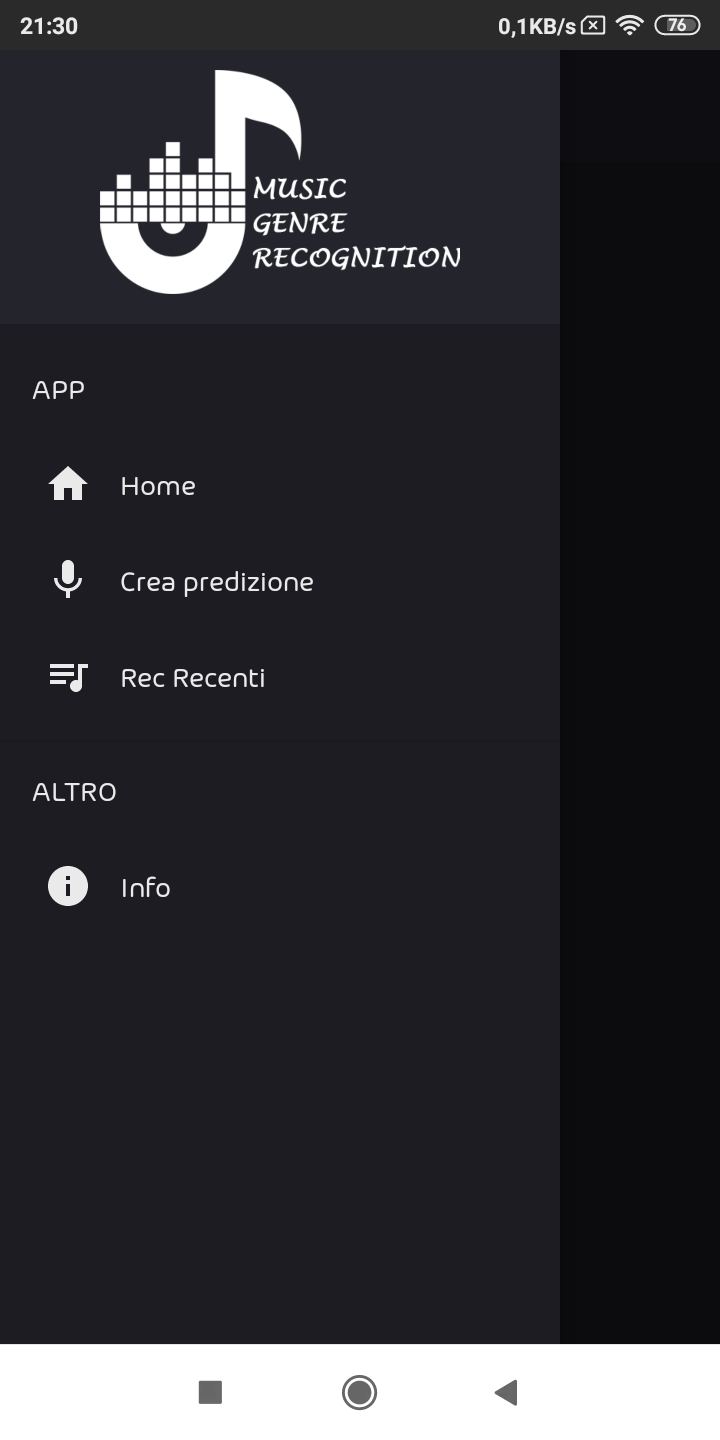
\includegraphics[scale=0.20]{./images/mobile01.jpg}
	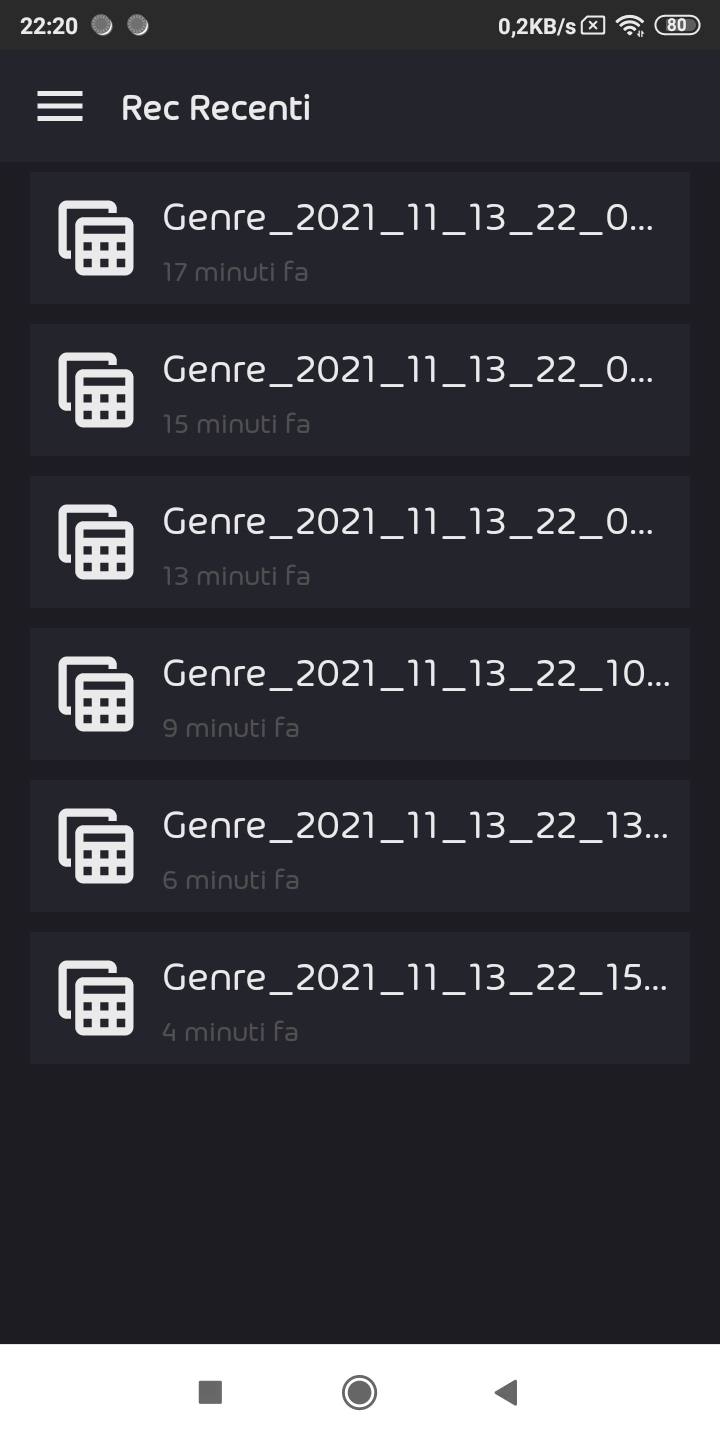
\includegraphics[scale=0.20]{./images/mobile02.jpg}
\end{figure}
\noindent Sono state create un paio di interfacce con elementi grafici ed è stato implementato un \textit{database} che tiene traccia del risultato delle registrazioni predette, in modo da poterle consultare anche in un secondo momento senza dover richiamare l'interprete di \textit{Tensorflow Lite}.\\
\newline
Per avviare la registrazione, basta cliccare sul pulsante centrale su cui è raffigurato un microfono. A questo punto il cellulare registra l'audio e per terminarla bisogna ricliccare sul pulsante.
\begin{figure}[H]
	\centering
	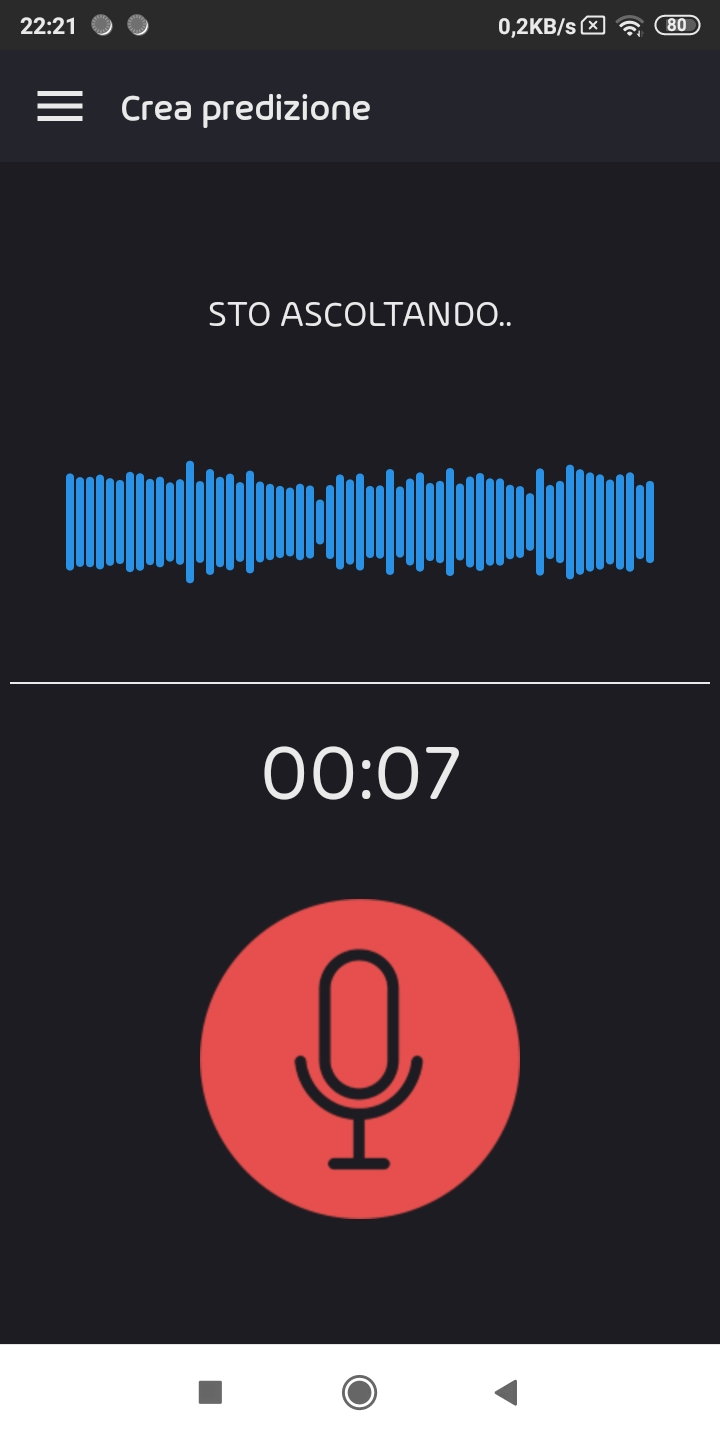
\includegraphics[scale=0.20]{./images/mobile03.jpg}
	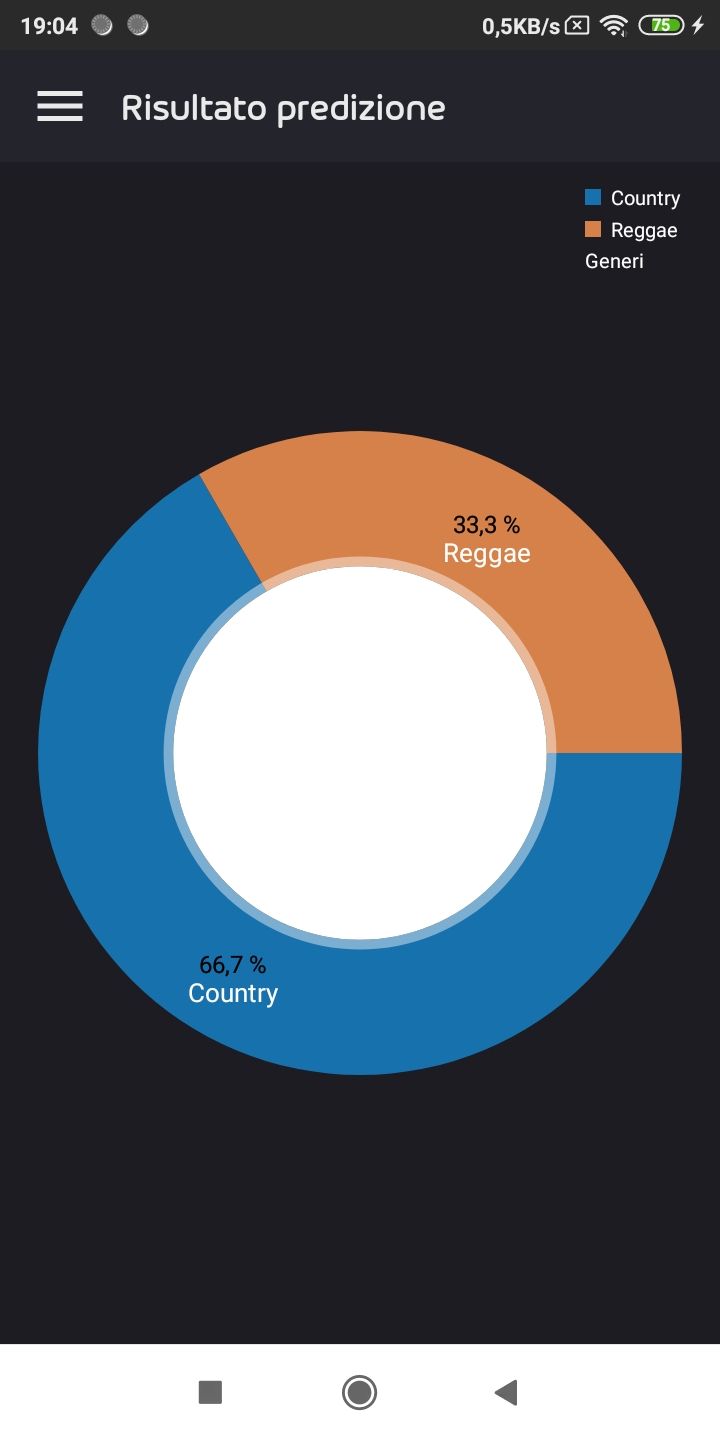
\includegraphics[scale=0.20]{./images/mobile04.jpg}
\end{figure}
\noindent A questo punto il file verrà salvato sul cellulare e convertito nel formato .\textit{wav}. Una volta aver ricavato le immagini dal \textit{file} audio, grazie al modello della rete è possibile avviare la predizione. Dopodiché il risultato apparirà in una nuova interfaccia.\\
\newline Per ricavare lo spettrogramma dalle registrazioni audio e per gestire la predizione è stato usato \textit{chaquopy}, un \textit{plugin} che consente di implementare codice \textit{Python} all'interno delle applicazioni \textit{Android}.

\subsection{Implementazione di Tensorflow Lite}
Una volta ottenuti gli \textit{input} della rete, possiamo eseguire l'inferenza con il modello.\\ Per predire correttamente il modello con l'albero decisionale è stato necessario creare una classe \textit{ModelNodeTree} che, essendo dinamica, funzioni con qualsiasi tipo e grandezza di albero.\\
Una volta passato il path del modello, relativo al nodo da predire, rendiamo accessibile l'interprete di \textit{Tensorflow Lite}, allochiamo i tensori ed estrapoliamo dal modello rispettivamente il tipo e il formato dell'\textit{input} e dell'\textit{output}. Passiamo il batch da predire tramite la funzione \textit{interpreter.set\_tensor()}, invochiamo l'interprete e tramite la funzione \textit{interpreter.get\_tensor()} otteniamo una copia dei valori provenienti dal tensore di \textit{output}.\\
In base al risultato, continuiamo la discesa dell'albero verso il ramo destro o sinistro, ricorsivamente, fino al nodo radice.
\vspace*{2ex}
\pythonexternal{./codes/mobile01.py}
\noindent Infine, i risultati vengono salvati in un \textit{JSON} e conservati nel \textit{database} dell'applicazione.
\vspace*{2ex}
\pythonexternal{./codes/mobile02.py}